\chapter{Reinforcement Learning}
\label{chap:reinforcementlearning}
This chapter describes an \ac{RL} approach, used to tackle the important problem of optimized trade execution. To a large extend, it is based on the \ac{RL} formulation, as described by Nevmyvaka \etal \cite{Nevmyvaka:2006}, but modified in detail.\\

\section{Original Algorithm}
The original algorithm claims to find optimal limits from a discretized state space, representing trade progress (\ie \emph{remaining time} and \emph{remaining inventory}) and additional market variables. While they achieved an impressive 50\% gain over more simple trading strategies, they left some room for improvements. As their work was based on a rather large, proprietary dataset of 1.5 years of millisecond time-scale limit order data from NASDAQ, it was furthermore intriguing to evaluate its performance on a smaller, self-recorded dataset of limited resolution.\\

Nevmyvaka \etal \cite{Nevmyvaka:2006} fused Q-learning and dynamic programming to learn a state-based strategy over the first year of their data in a brute force manner.

\subsection{State space}
\label{chap:statespace}
The state space consists of various discrete variables, describing the current trade progress (\emph{private variables}) and the current market situation as observable from orderbook data (\emph{market variables}). The two private variables \lstinline!time! and \lstinline!volume! make the base for all subsequent experiments, while various additional market variables were enclosed to examine their impact on a valuable decision making.\\

As such, each \lstinline!state! $s \in <time, volume ,o_1, o_2, ...>$ forms a vector of at least two private variables, plus a variable number of market variables. More specifically, the following market variables were evaluated in terms of improvement over a state space based on two private variables only.
\begin{description}
\item[Bid-Ask Spread]: spread between best bid price and best ask price.
\item[Bid-Ask Volume Misbalance]: volume imbalance between orders at the best bid price and the best ask price.
\item[Immediate Market Order Cost]: costs, if remaining volume would be executed immediately, at the current market price.
\item[Signed Transaction Volume]: signed volume of all trades executed within last 15 seconds. A positive value indicates more buy orders, while a negative value complies to more sell orders being executed.
\end{description}

All market variables were discretized into 0 (low), 1 (medium) and 2 (high), while the concrete category mapping process was not further described.

\subsection{Action space}
\label{chap:actionspace}
Actions define the level of trading aggression to be performed. An action $a \in \mathbb{R}$ defines the deviation between current best price and chosen limit price, as $bid + a$ (for buy orders) and $ask - a$ (for sell orders).\\

In case of the market situation as shown in \Cref{table:orderbook:example:again}, a buy order with an aggressive action $a=1.4$ would translate into $limit=28.7+1.4=30.1$. This limit would allow trading up to 75 shares instantaneously.\\

\begin{table}
\centering
\begin{tabular}{lrlrrr}
\toprule
{} &  Amount &    Type &  Volume &  VolumeAcc &  norm\_Price \\
\midrule
31.00 &   200.0 &     ask &  6200.0 &     8425.0 &    1.074533 \\
30.00 &    50.0 &     ask &  1500.0 &     2225.0 &    1.039871 \\
29.00 &    25.0 &     ask &   725.0 &      725.0 &    1.005208 \\
28.85 &     NaN &  center &     NaN &        NaN &         NaN \\
28.70 &   200.0 &     bid &  5740.0 &     5740.0 &    0.994810 \\
28.50 &   100.0 &     bid &  2850.0 &     8590.0 &    0.987877 \\
28.00 &   300.0 &     bid &  8400.0 &    16990.0 &    0.970546 \\
\bottomrule
\end{tabular}
\caption{Action $a=1.4$ translates into $limit=28.7 + 1.4 = 30.1$.}
\label{table:orderbook:example:again}
\end{table}

The employed number of selectable actions and their actual value range is not further specified.


\subsection{Costs}
\label{chap:costs}
Costs are defined as the slippage induced from the previously chosen action. The baseline is given by the initial center price. The following formula is used to compute (partial) costs in terms of price deviation from the idealized case of buying all shares at the initial center price:
\begin{equation}
   cost = (avg\_paid - initial\_center) * volume\_traded
\end{equation}
\begin{equation}
   initial\_center = (\dfrac{ask_t+bid_t)}{2} | t=0
\end{equation}

Since the complete trade execution happens within a finite time horizon and full execution of the \lstinline!volume! is mandatory, partial costs, as observed after the individual \lstinline!trading_periods!, can simply be summed up without any discounting.


\subsection{Backward learning}
\label{chap:backwardlearning}
In order to learn the optimal limit for each possible situation, orderbook windows are examined in a backward, brute-force manner as described in \Cref{lst:bruteforce:pseudocode}. Each orderbook window from the training data set is sampled $T*I*L$ times, where $T$ is the number of performed limit revisions, $I$ is the number of discrete volume states and $L$ is the number of available actions.

\begin{lstlisting}[frame=single, breaklines=true, basicstyle=\scriptsize, caption=Brute-Force strategy learning approach as described in \Cite{Nevmyvaka:2006}., label=lst:bruteforce:pseudocode]
Optimal_strategy(V, H, T, I, L)
    For t=T to 0
        While(not end of data)
            Transform (orderbook) -> o_1 ... o_R
            For i =0 to I
                For a = 0 to L
                    Set x = [t, i, o_1, ..., o_R]
                    Simulate transition x -> y
                    Calculate immediate cost_im(x, a)
                    Look up argmax cost(y, p)
                    Update cost([t, v, o_1, ..., o_R], a)
    Select the highest-payout action argmax cost(y, p) in every state y to output optimal policy
\end{lstlisting}

While the algorithms running time depends solely on the resolution of the two private variables, the chosen action space and the size of the training data, it is approximately independent of the number of market variables chosen. The transition simulation was not further described, but for this thesis the model described in \Cref{chap:tradeexecution} is utilized. The cost update rule is given below: 
\begin{equation}\label{eq:costfunction}
   cost(x_t, a) = \dfrac{n}{n+1} cost(x_t, a) + \dfrac{1}{n+1} [cost_{im}(x_t,a) + \arg\min_{p}cost(x_{t-1}, p)]
\end{equation}

The algorithm assumes the individual trading\_periods to be of an (approximately) Markovian nature, where the optimal action to choose at a state with $t = \tau$ is completely independent of actions chosen previously ($t \geq \tau$).\\

As such the state-action function can be computed inductively via dynamic programming. In a first round, expected costs for all actions in states being immediate predecessors of end states (\ie $t=1$) are computed according to \Cref{eq:costfunction}. \Cref{fig:heatmap:t1} visualizes the resulting optimal costs (right) and corresponding actions (left) after the first round has finished.

\begin{figure}[ht]
	\centering
   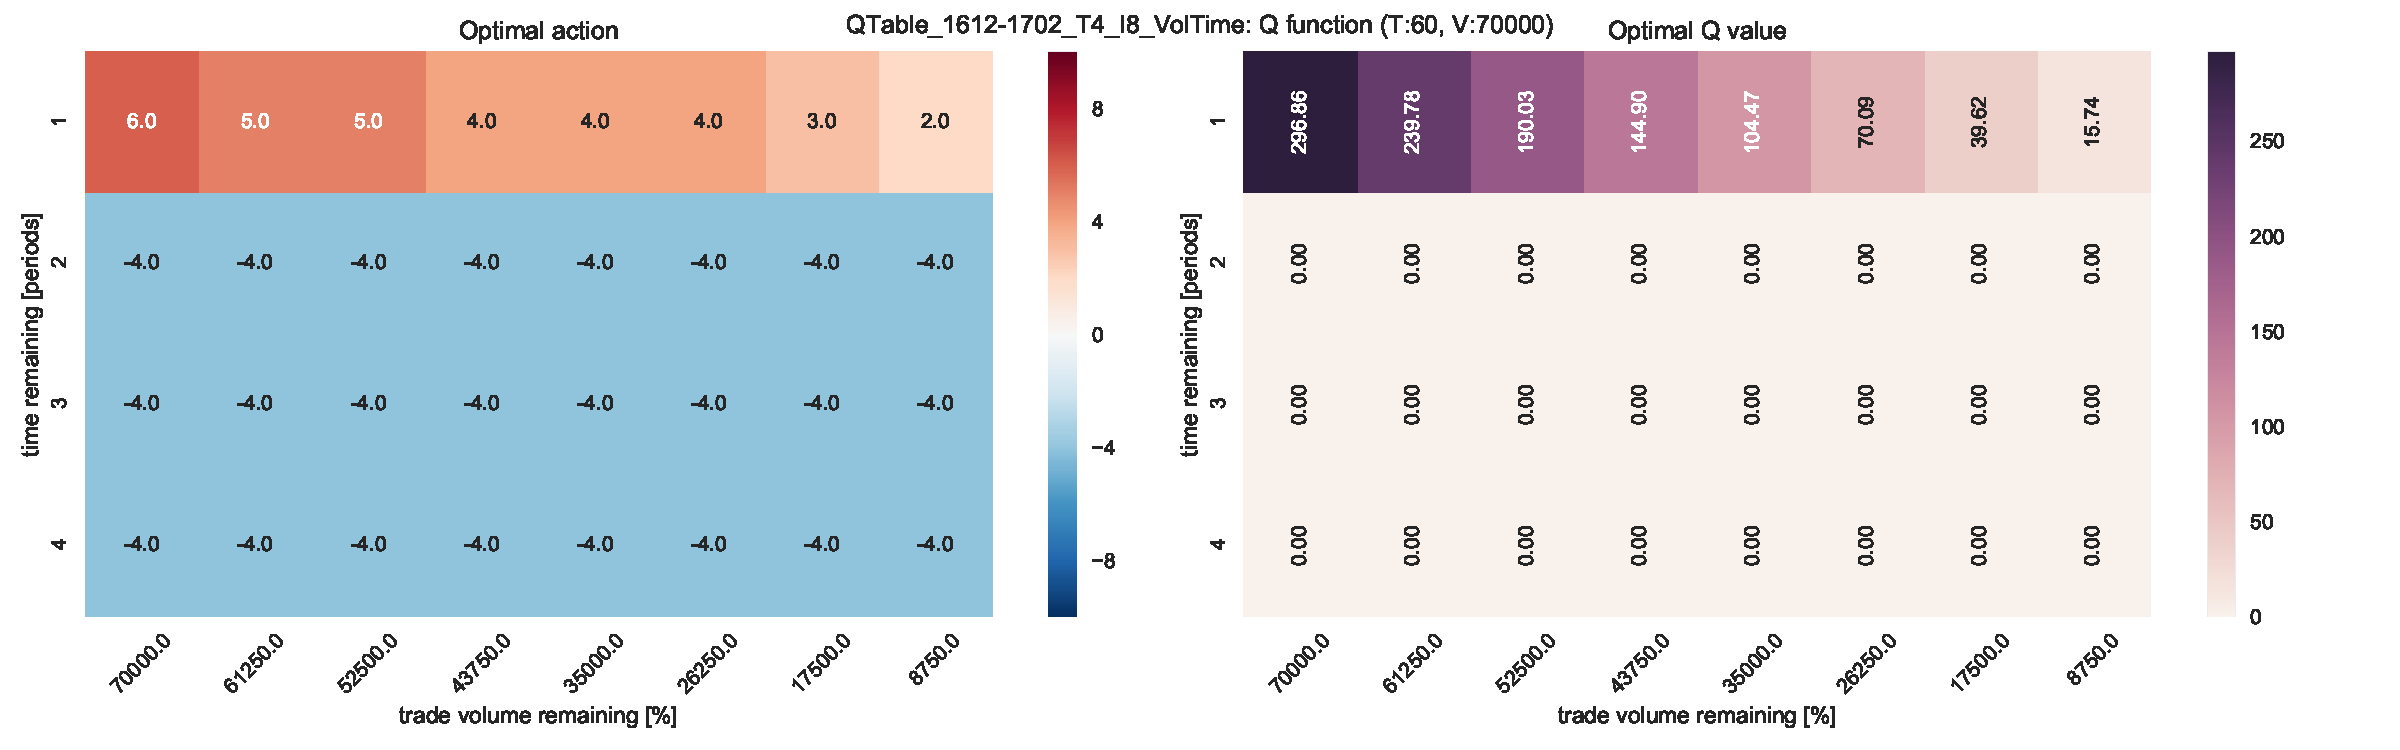
\includegraphics[width=1.\textwidth]{content/drawings/heatmap_3months_t1}
	\caption{State-Action function, visualized after the first training round.}
	\label{fig:heatmap:t1}
\end{figure}

Knowing the optimal state action values for all states with $t=1$, all informations are given to compute the optimal state action values for their predecessor states with $t=2$ (see \Cref{fig:heatmap:t2}).

\begin{figure}[ht]
	\centering
   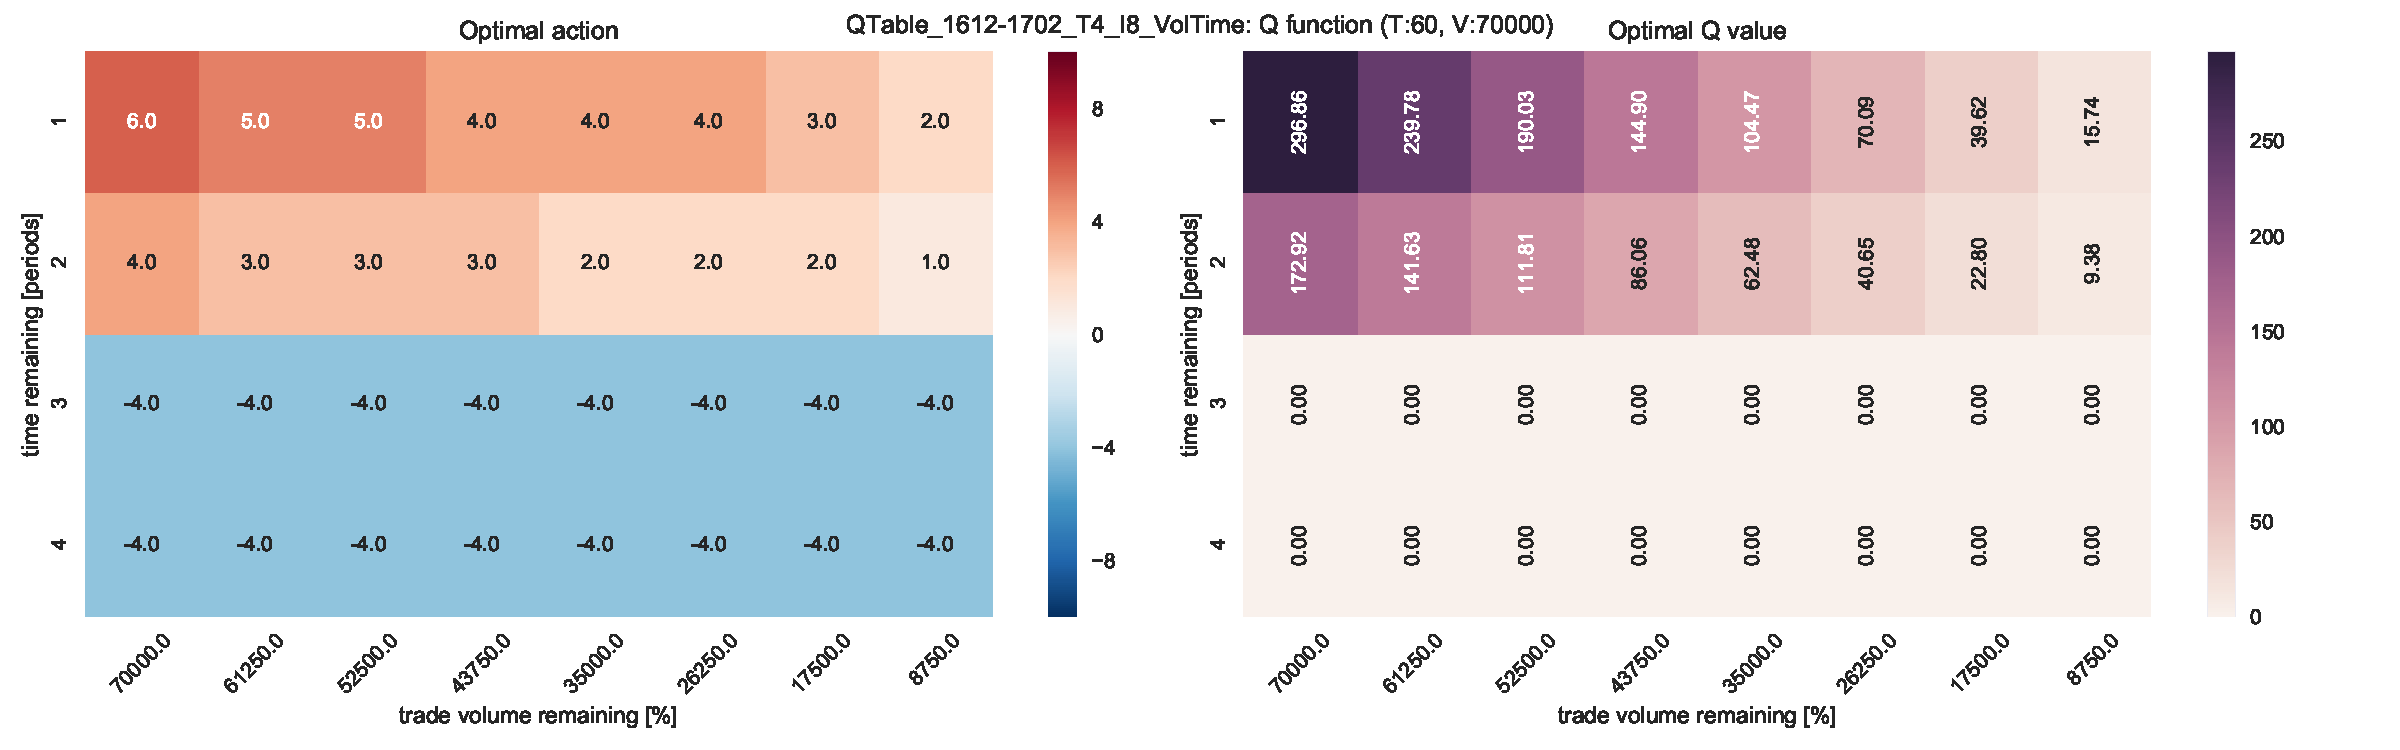
\includegraphics[width=1.\textwidth]{content/drawings/heatmap_3months_t2}
	\caption{State-Action function, visualized after the second training round.}
	\label{fig:heatmap:t2}
\end{figure}

After $T=4$ iterations, a globally optimal policy as shown in \Cref{fig:heatmap} has been found. This example was learned from 4154 orderbook windows\footnote{Orderbook windows of 60 minutes, as extracted from USDT\_BTC data between Nov, 10th 2016, 10am until Mai, 31st 2017}, where $70.000\$$ cash (discretized in 8 intervals) had to be traded into Bitcoins. The annotated q value (right) give the corresponding minimum over all available actions only.

\begin{figure}[ht]
	\centering
   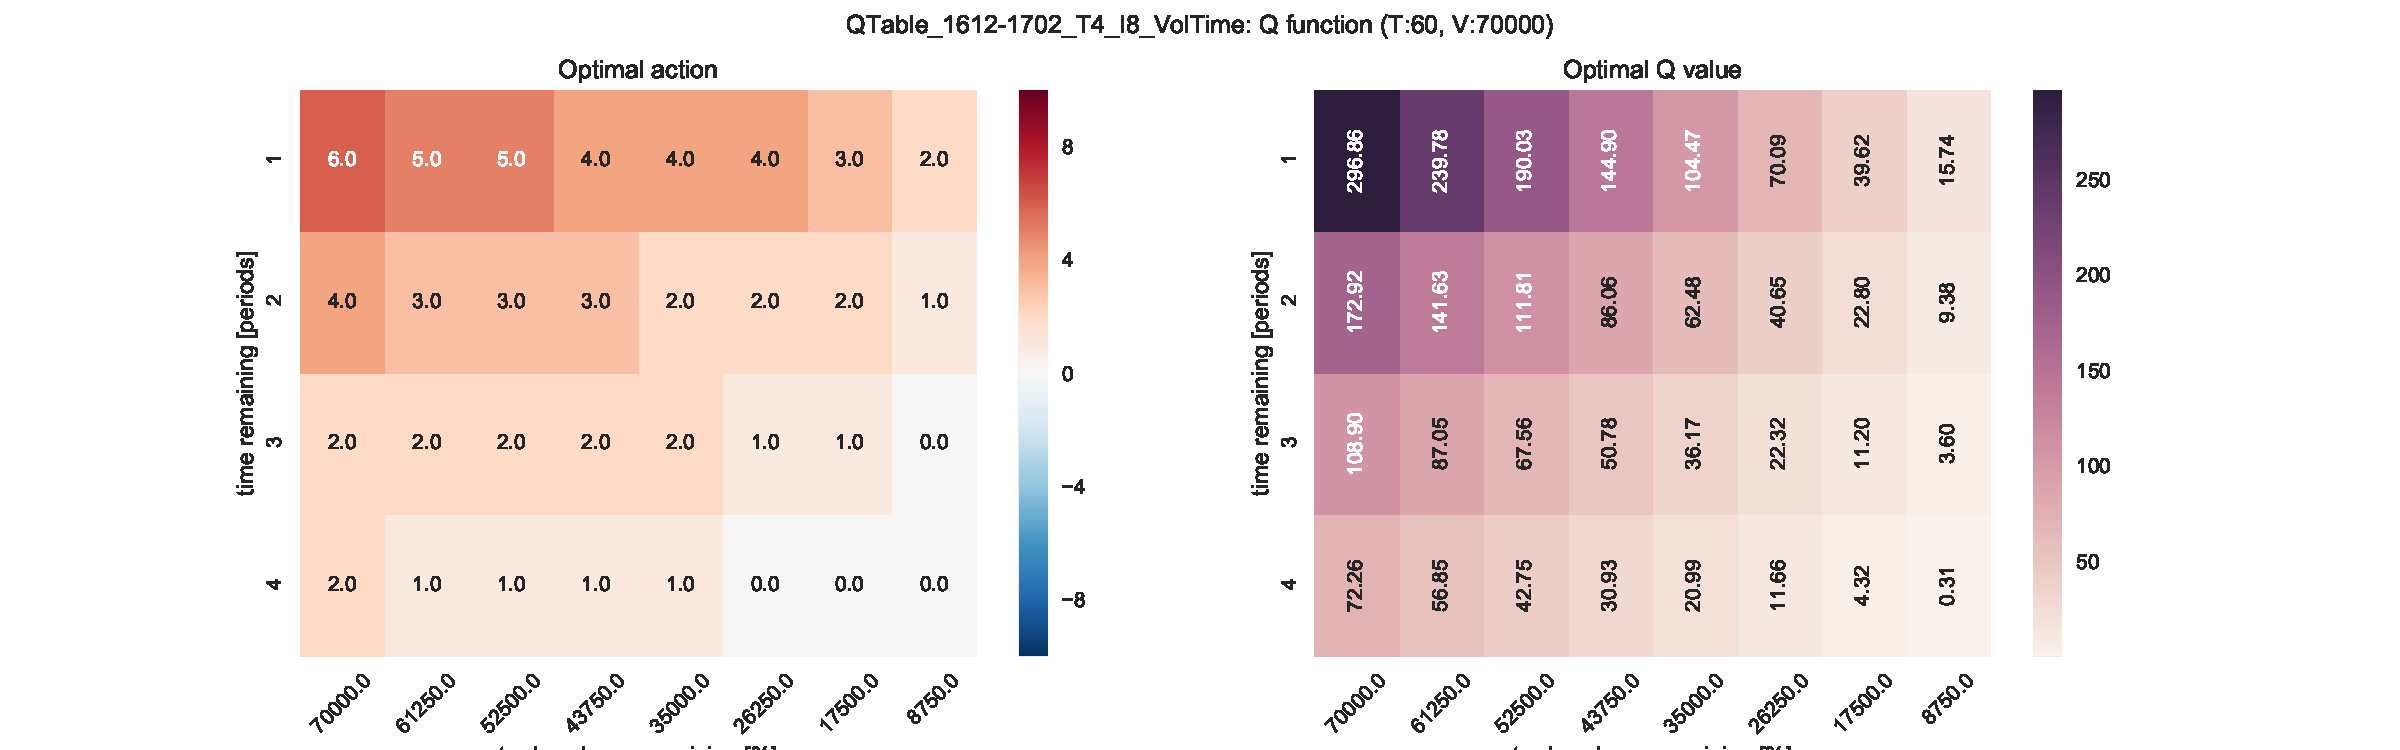
\includegraphics[width=1.\textwidth]{content/drawings/heatmap_3months}
	\caption{Final State-Action function.}
	\label{fig:heatmap}
\end{figure}

\Cref{fig:heatmap} illustrates clearly, how the optimal strategy becomes more aggressive as time ceases and a large portion of the trading volume remains unexecuted.

\subsection{Discussion}
\begin{itemize}
\item Discrete Actions
\item Discrete States (why 3 bins?, borders?, \ldots{}) / Lookup-table / Rounding-issues
\item Vulnerable to seldom observed market states

\item Why crossing the spread?! Start from ask, rather than bid!\\
Influence/dependence on Spread (+8\% claimed!) as MarketVariable seems obvious here.
\end{itemize}


\section{Improvements}
\begin{itemize}
\item actions represent deviation from ask, not bid
\item Forward Sampling
\begin{itemize}
\item Growing batch learning
\item Experience Replay (NN\_Agent)
\item Exploration vs avoidance of repeatedly trying same actions.
\end{itemize}
\begin{itemize}
\item Markov Property violated
\item Realistic samples, no rounding. Better fit for \emph{curious} masterbook shapes as described in \Cref{chap:modelcorrectness}?!
\end{itemize}
\item Function Approximation
\begin{itemize}
\item RandomForest (BatchTree Agent)
\item NN Agent
\end{itemize}
\item Different Market Variables:
\begin{itemize}
\item Immediate Slippage/MarketPrice Imbalance
\item MarketPrice Spread (buy vs. sell)
\end{itemize}
\item Cost function
\begin{itemize}
\item Slippage based on initial\_center
\item Improvement over MarketPrice??
\end{itemize}
\end{itemize}

\section{RL Agents}
bla

\subsection{QTable Agent}
bla

\subsection{BatchTree Agent}
bla

\subsection{NN Agent}
bla

\cleardoublepage{}